% #########################################################################
% #               METODOLOGÍAS Y TÉCNICAS DE INVESTIGACIÓN                #
% #########################################################################

% Definición de nombres
\newcommand{\estudiante}{García Justel, Alan}
\newcommand{\titulo}{MÁSTER EN INGENIERÍA COMPUTACIONAL Y SISTEMAS INTELIGENTES}
\newcommand{\asignatura}{ROBÓTICA}
\newcommand{\portada}{ROBOTIKA/images/portada_robotika.jpg}
\newcommand{\colorportada}{title_red}
\newcommand{\curso}{2024-2025}



% Notebook
\begin{document}

\newgeometry{bottom=2cm}

\begin{titlepage}
    % Logo de la universidad
    \begin{textblock*}{\textwidth}(2cm,0.4cm)
        \begin{center}
            \begin{minipage}{0.45\textwidth}
                \centering
                
\includegraphics[width=\textwidth]{common/Logo_EHU.jpg}
            \end{minipage}\hfill
            \begin{minipage}{0.45\textwidth}
                \centering
                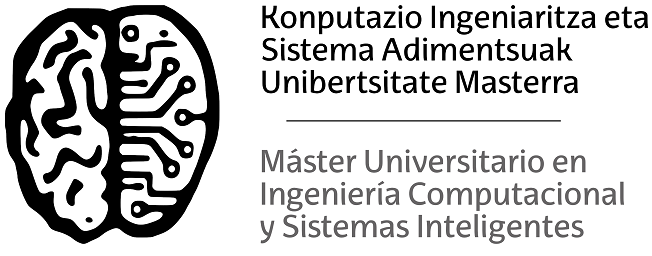
\includegraphics[width=0.8\textwidth]{common/Logo_KISA.png} 
            \end{minipage}
        \end{center}
    \end{textblock*}
    
    % Franja de color
    \begin{tikzpicture}[remember picture, overlay]
        \fill[\colorportada] (current page.north west) ++ (0,-3.01cm) rectangle (\paperwidth,-3cm);
    \end{tikzpicture}
    
    \begin{textblock*}{\paperwidth}(\dimexpr\parindent+\oddsidemargin+3em\relax,3.5cm)
        \begin{minipage}{\dimexpr\linewidth-7.5cm\relax}
            \color{white}
            \noindent\rule{\linewidth}{0cm}
            \textsf{ {\large \titulo}}
            \newline
            \newline \newline
            \textsf{\textbf{ {\Huge APUNTES DE ASIGNATURA }}}
        \end{minipage}
    \end{textblock*}
    
    % Nombre asignatura
    \vspace*{3.5cm}
    \begin{minipage}{\linewidth}
        \setlength{\baselineskip}{1.7\baselineskip}
        \centering
        \textsf{ \textbf{ {\LARGE \asignatura }}}
    \end{minipage}

    % Foto de portada
    \vspace*{0.5cm}
    \begin{figure}[H]
        \centering
        \includegraphics[width=10cm, height=8cm]{\portada}
    \end{figure}

    
    
    % Estudiante
    \vspace{0.2cm}
    \noindent {\footnotesize \textbf{Estudiante:} \estudiante}
    \newline
    \noindent\makebox[\linewidth]{\rule{\textwidth}{0.4pt}} % Línea horizontal

    % Curso y Fecha
    \vspace{0.1cm}    
    \noindent {\footnotesize \textbf{Curso: } \curso \hfill \textbf{Fecha:} \today }
\end{titlepage}

\restoregeometry
\setcounter{figure}{0} % Incluimos el título
\newpage

% Índices
\tableofcontents\thispagestyle{empty} %\newpage
% \listoffigures\thispagestyle{empty}   %\newpage
% \listoftables\thispagestyle{empty}    %\newpage
\newpage

\section{Playing with robots: issues and experiences}
Jugar es una actividad fundamental para aprender, entrenar o entretenerse, y jugar con robots facilita su integración en entornos cotidianos. Para que un robot participe en un juego, debe seguir sus reglas, evitando interacciones ineficaces o artificiales. Sin embargo, existen desafíos clave, como la capacidad de respuesta en tiempo real, la interacción con usuarios frágiles (niños o personas con discapacidad) y cuestiones éticas relacionadas con su uso.

Cada año, millones de robots ingresan al mercado de los juguetes, aunque ninguno tiene aplicaciones profesionales. Su precio es inferior a 200€, lo que impone limitaciones de hardware. Comparados con los juguetes tradicionales, los robots comparten aspectos como la forma, los materiales y la posibilidad de manipulación, pero deben enfrentar retos adicionales: la calidad del movimiento, el ruido asociado y la simplicidad de sus sensores y reacciones. Se espera que en el futuro los robots de juguete sean capaces de interpretar señales implícitas, tomar la iniciativa, mantener la atención del usuario y seguir siendo de bajo costo.

Existen diversas formas de jugar con robots: competitivo o cooperativo, primera persona o mediante avatares, juegos físicos o cognitivos, así como diferentes tipos de juego según las reglas y objetivos: juego libre, de práctica, de simulación, de construcción o basado en reglas. En la interacción humano-robot (HRI), hay factores clave a considerar. Primero, la sensación de seguridad, ya que los robots deben ser percibidos como seguros en tamaño y velocidad. Segundo, la justicia, asegurando que el robot siga las reglas y tenga un nivel de habilidad adecuado. Tercero, la participación activa, garantizando que el juego sea desafiante y motivador sin ser demasiado fácil o difícil. Finalmente, el canal de interacción, ya que la comunicación entre humano y robot debe ser clara y efectiva.

Ejemplos de interacción en juegos incluyen el \textit{Jedi Game}, donde un dron actúa como un droide y el jugador debe defenderse de ataques láser, y el \textit{Robotower}, donde humano y robot compiten por presionar primero un botón en una arena de juego. 

Otro aspecto crucial es la inclusión en el juego, permitiendo que cualquier persona, sin importar sus capacidades, pueda jugar, aprender y divertirse. Un juguete es cualquier objeto que genere interés, y este interés se logra ofreciendo novedad, exploración y opciones de configuración. Actualmente, existen juguetes para niños con desarrollo típico, juguetes adaptados para personas con discapacidad, juguetes específicos para discapacitados y juguetes diseñados para todos.

Finalmente, se han identificado diversas líneas de investigación abiertas para mejorar la experiencia de juego con robots: modelado en tiempo real del usuario, adaptaciones en línea, interacciones físicas según lenguaje y emociones, y dinámicas de juego.  
\newpage

\section{Social Media Mining or Human-Robot Interaction}
El modelado semántico ha permitido desarrollar herramientas de visualización que clasifican datos de manera intuitiva. Un ejemplo es la recolección y análisis de tweets mediante herramientas que facilitan la identificación de patrones en los mensajes. La visualización semántica permite representar datos de forma clara y comprensible, como en los \textit{treemaps}, donde al hacer clic en un concepto se despliegan subtemas relacionados. Estas herramientas han sido aplicadas en contextos críticos como la protección civil, facilitando la navegación en grandes volúmenes de datos. Un caso concreto fue el atentado de París, donde se detectó un movimiento ciudadano en redes sociales ofreciendo refugio, lo que permitió coordinar mejor la ayuda.

Por otro lado, la visualización inmersiva busca mejorar la comprensión a través de entornos amplios de 360º con elementos 3D y 2D, simulando espacios de aprendizaje interactivos. Se ha demostrado que este tipo de herramientas pueden mejorar la enseñanza en entornos escolares al permitir una interacción más profunda con los conceptos analizados.

El proyecto \textit{Social Media Mining for Human-Robot Interaction} investiga cómo mejorar la interacción entre humanos y robots sociales a partir de la información publicada en redes sociales. Uno de los principales desafíos es la comunicación entre el usuario y el robot, ya que la interacción debe ser natural y atractiva. Los robots sociales están diseñados para comunicarse tanto verbal como físicamente, lo que resulta especialmente útil en iniciativas como la asistencia a personas mayores. Estos robots pueden supervisar la medicación, el bienestar emocional, contactar a familiares o servicios de emergencia, y ofrecer entretenimiento o entrenamiento cognitivo. En muchos casos, la interacción con un robot resulta más accesible para personas mayores que el uso de un \textit{smartphone} o una \textit{tablet}. La confianza del usuario es clave para la adopción de estos robots, por lo que su utilidad debe ser clara en todo momento.

Un ejemplo destacado es el robot social \textit{Mini}, que utiliza expresiones visuales y una \textit{tablet} como vía alternativa de interacción. Sus principales funciones incluyen entretenimiento (contar chistes, dar noticias o recomendaciones) y terapia cognitiva (ejercicios de memoria, reconocimiento de objetos, juegos de lenguaje). Para evitar la repetición en los diálogos, \textit{Mini} personaliza la generación de contenido según el perfil del usuario, extrayendo información relevante de redes sociales como Twitter y adaptándola a sus intereses. Además, incorpora comunicación no verbal mediante movimientos y cambios de color que reflejan su estado de ánimo. En algunas interacciones, el robot simula estar pensando para mantener la atención del usuario mientras procesa la información.

Las pruebas con personas mayores han recibido críticas mayormente positivas, aunque se ha señalado que existen retrasos en la interacción. Como conclusiones, se identificó la necesidad de mejorar la velocidad de procesamiento y automatizar la generación de perfiles. A pesar de estos desafíos, las pruebas indicaron que los usuarios percibían las interacciones como naturales, lo que sugiere que el robot se adapta eficazmente a cada persona.
\newpage

\section{Aplicaciones en robótica inndustrial}
Un robot debe de ser capaz de percibir el entorno, planificar los movimientos y ejecutarlos con algoritmos de control. En el departamento de navegación autónoma de Tekniker se enfocan en movilidad, manipulación, interacción y percepción. La manipulación de objetos es una capacidad clave, que abarca desde la percepción del objeto hasta la planificación de la trayectoria para manipularlo, considerando la variabilidad de los objetos, como su forma, peso y material. Sin embargo, las soluciones actuales tienen limitaciones en flexibilidad y adaptabilidad. 

En la aplicación de bin-picking, se busca manipular una caja y vaciarla de piezas industriales, utilizando un sistema de adquisición de imágenes, segmentación de escenas, estimación de poses e identificación de puntos de agarre. Para entrenar los modelos de segmentación, utilizan simulaciones en Unity con modelos CAD y ajustan los hiperparámetros automáticamente mediante una herramienta evolutiva como Raylib. La automatización del proceso de selección del punto de agarre se realiza mediante modelos de deep learning, y la evaluación de estos puntos se realiza en simuladores como Mujoco, con pruebas en entornos reales. Un desafío importante es el salto entre simulación y realidad, por lo que se utilizan algoritmos metaheurísticos para ajustar el movimiento simulado al real. 

En cuanto a la toma de decisiones sobre qué objeto manipular, se emplea un módulo basado en IA entrenado mediante aprendizaje por refuerzo para crear políticas de agarre, modelado como un Deep Q-Learning. Dado que las piezas pueden ser desconocidas, se entrenan modelos específicos para estas situaciones. Para la programación de robots, se utilizan árboles de comportamiento, inspirados en los videojuegos, que permiten la reutilización de bloques y facilitan la visualización del flujo del programa. También se investiga el aprendizaje por demostración, en el que el robot aprende a generar árboles de comportamiento. En la fase de agarre, se utilizan ventosas para formas regulares, pinzas para piezas irregulares y magnetismo para piezas metálicas. Además, se emplean imágenes visuotáctiles para evaluar la efectividad del agarre.

En el campo de la navegación autónoma, Teknikbot, un robot de Tekniker, realiza navegación en espacios basados en mapas 2D utilizando ROS y sensores para la localización. Mainbot, diseñado para el mantenimiento de parques solares, utiliza un sistema RTK para la localización. Coinspect inspecciona alas de avión usando un sistema de visión que calcula la relación de la posición entre el robot y el ala. Greenpatrol, enfocado en el tratamiento de plantas, utiliza deep learning para identificar plagas.

Respecto a la interacción persona-robot, se utiliza la detección de gestos, donde las coordenadas de los puntos de la mano sirven como input para un modelo de clasificación. Además, se emplean combinaciones de interacciones por voz y gestos para eliminar ambigüedades, como en el caso de un robot que debe "coger algo" cuando se le señala. La programación de robots mediante realidad virtual está diseñada para la enseñanza y entornos industriales, permitiendo la interacción mediante un chatbot o un gemelo digital con gafas de realidad aumentada. De este modo, se pueden definir y ejecutar movimientos del robot virtualmente. Además, se han entrenado clasificadores para identificar la necesidad de ayuda de una persona en entornos colaborativos mediante la monitorización de la mirada y el comportamiento.

En el ámbito de los robots industriales, se implementa la detección de humanos y puntos clave mediante OpenPose, añadiendo este detector al sistema de proximidad del robot para que se detenga si una persona entra en su área de operación. Además, en seguridad en entornos industriales, se controla una apisonadora mediante detección de intenciones humanas, con un sistema BEV que avisa a las personas si entran en áreas peligrosas.
\newpage

\section{Measuring Animation Quality}
La animación de agentes virtuales, o representaciones humanoides digitales, presenta algunas ventajas con respecto a los robots ya que no están sujetos a limitaciones físicas y, por tanto, presentan un rango de movimiento más amplio. Sin embargo, medir la calidad de la animación es un reto considerable, ya que existen métricas objetivas y subjetivas. Las métricas objetivas proporcionan resultados consistentes, pero las métricas subjetivas dependen de la percepción de las personas, lo que puede variar. En este sentido, se presentan los desafíos de evaluación de la calidad de los movimientos generados por algoritmos automáticos, como el GENEA challenge, que tiene como objetivo generar gestos a partir del habla. Esta tarea es compleja debido a que existen múltiples gestos posibles para una misma frase, la falta de datos para entrenamiento y las diferencias individuales entre las personas.

Con el objetivo de unificar y comparar distintos algoritmos y técnicas de generación de movimiento se creó el GENEA Challenge 2022, que utilizó un conjunto de datos de 20 horas de audio y 3D de movimiento y contó con la participación de empresas como Ubisoft y Huawei. Se registraron 10 presentaciones finales, y los participantes recibieron calificaciones de los animadores lo que permitió generar un ranking subjetivo. Este estudio mostró que, aunque las opiniones individuales diferían, los resultados eran generalmente consistentes. La evaluación también reveló que todas las soluciones propuestas eran superiores al modelo base del benchmark y los resultados mostraron que las métricas objetivas no se correlacionaban de manera significativa con las métricas subjetivas, lo que indica que aún se necesita mejorar la definición de métricas objetivas para medir la calidad de los gestos. Además, el ganador del desafío no usó redes neuronales profundas sino que se basó en sistema de grafos que conectaba datos reales de manera inteligente según el discurso.

Por otro lado, actualmente es muy común realizar capturas de moviento de actores humanos para generar las animaciones de los agentes virtuales. Sin embargo, en este proceso es común que existan marcadores perdidos en las grabaciones y como la captura de movimiento tradicional es costosa, se han desarrollado técnicas de reconstrucción de los datos. En este proceso, se utilizan métricas objetivas como el error cuadrático medio (MSE), la preservación de la distancia entre huesos y la distancia en las velocidades. Además, se ha observado que el sistema de reconstrucción obtiene mejores resultados al realizarlo de forma jerárquica, comenzando con la predicción de las caderas, luego del torso y, finalmente,  la cabeza y los miembros, lo que mejora los resultados frente a la predicción simultánea de todo el movimiento.

Los resultados subjetivos mostraron que la estrategia jerárquica era eficaz, mientras que las métricas objetivas no coincidían bien con las percepciones subjetivas. Por ejemplo, si un marcador se movía un centímetro, las métricas objetivas registraban una diferencia significativa, mientras que las evaluaciones subjetivas consideraban que la secuencia seguía siendo adecuada. Aunque algunas métricas objetivas mostraron correlaciones aceptables con las evaluaciones subjetivas, el RMSE (Root Mean Square Error) no fue el mejor indicador para esta tarea. En general, las métricas objetivas deben considerar la cohesión espacial y temporal del movimiento para lograr una evaluación más precisa de la calidad.
\end{document}